% !TeX program = lualatex
% !TeX encoding = utf8
% !TeX spellcheck = uk_UA
% !BIB program = bibler

\documentclass[onlytextwidth]{beamer}
\usetheme{Electromagnetism}
\usepackage{Electromagnetism}
\usepackage[europeanresistors, americaninductors]{circuitikz}
\usepackage{tikz-3dplot}


%============================================================================
\title[Лекції електрики та магнетизму]{\huge\bfseries Явище електромагнітної індукції}
\subtitle{Лекції з електрики та магнетизму}
\author{Пономаренко С. М.}
\date{}
%============================================================================
\graphicspath{{pictures/}}
\begin{document}
\begin{frame}[plain]
	\maketitle
\end{frame}

% ============================== Слайд ## ===================================
\begin{frame}{Зміст}{}
	\tableofcontents
\end{frame}
% ===========================================================================



%% --------------------------------------------------------
\section{Явище електромагнітної індукції}
%% --------------------------------------------------------



% ============================== Слайд ## ===================================
\begin{frame}{Явище електромагнітної індукції}{}
	\begin{block}{Явище електромагнітної індукції (Фарадей)}\justifying
		У 1831 р. Фарадеєм було зроблено одне з найбільш фундаментальних відкриттів в електродинаміці --- \alert{явище електромагнітної індукції}. Воно
		полягає в тому, що в замкненому провідному контурі при зміні магнітного потоку, охопленого цим контуром, виникає електричний струм --- його назвали
		індукційним.
	\end{block}

	\vfill

	\href{https://youtu.be/GrBYG8NIUoU}{\color{blue}\small Досліди Фарадея}

\end{frame}
% ===========================================================================



% ============================== Слайд ## ===================================
\begin{frame}{Закон електромагнітної індукції}{}
	\begin{block}{}\justifying
		Електрорішійна сила (ЕРС), що виникає в контурі пропорційна швидкості зміни магнітного потоку, що пронизує площу, охоплену даним контуро:
		\begin{equation*}
			\tcbhighmath{\mathcal{E}_\text{ind} =  -\frac1c \frac{d\Phi}{dt}} = -\frac1c \frac{d}{dt} \iint\limits_S \Bfield\cdot\vect{S}.
		\end{equation*}
	\end{block}
	\begin{columns}
		\begin{column}{0.5\linewidth}\centering
			\begin{tikzpicture}[rotate=90, scale=0.9, >=latex, midarrow/.style={%
							postaction={ decorate,
									decoration={ markings, mark=at position .7 with {\arrow{latex}}}}}]
				\begin{scope}%[rotate around={45:(0,1)}]
					\draw[arrowpos={0.5}{2pt}{7pt}, red!40, ultra thick] (1.1,0) [partial ellipse=360:0:0.3 and 1];
				\end{scope}

				\foreach \y in {-3,...,3}{
						\draw[blue, midarrow] plot[domain=1:3] (\x, 0.2*\y+0.05*\y*\x^2);
					}
				\node[blue, font=\small] at (3.5, 0) {$\frac{d\Phi}{dt}>0$};
			\end{tikzpicture}
		\end{column}
		\begin{column}{0.5\linewidth}\centering
			\begin{tikzpicture}[rotate=90, scale=0.9, >=latex, midarrow/.style={%
							postaction={ decorate,
									decoration={ markings, mark=at position .7 with {\arrow{latex}}}}}]
				\begin{scope}%[rotate around={45:(0,1)}]
					\draw[arrowpos={0.5}{2pt}{7pt}, red!40, ultra thick] (1.1,0) [partial ellipse=0:360:0.3 and 1];
				\end{scope}

				\foreach \y in {-3,...,3}{
						\draw[blue, midarrow] plot[domain=1:3] (\x, 0.2*\y+0.05*\y*\x^2);
					}
				\node[blue, font=\small] at (3.5, 0) {$\frac{d\Phi}{dt}<0$};
			\end{tikzpicture}
		\end{column}
	\end{columns}
	\begin{block}{Правило Ленца}\justifying\small
		Індукований струм має такий напрямок, щоб за допомогою
		створюваного ним магнітного поля перешкоджати зміні
		магнітного потоку, тобто щоб послабити дію причини, яка збуджує
		цей струм.
	\end{block}
\end{frame}
% ===========================================================================


% ============================== Слайд ## ===================================
\begin{frame}{Струми Фуко}{}
	\begin{block}{}\justifying
		Струми Фуко --- вихрові індукційні струми, які виникають у провіднику під час зміни магнітного потоку через поверхню провідника.
	\end{block}
	\begin{center}
		\includegraphics[width=.5\linewidth]{Fuko_currents}
	\end{center}

	\begin{block}{}\justifying
		Струми Фуко, як і індукційні струми в лінійних провідниках, підпорядковані правилу Ленца: їх магнітне поле направлене так, щоб протидіяти змінам
		магнітного потоку, що індукували ці струми.
	\end{block}
\end{frame}
% ===========================================================================


% ============================== Слайд ## ===================================
\begin{frame}{Закон збереження магнітного потока}{}\small
\begin{block}{}
    Нехай замкнутий виток з опором $R$ перебуває в зовнішньому магнітному полі.
\end{block}
\vspace*{-2ex}
	\begin{columns}
		\begin{column}{0.2\linewidth}
			\includegraphics[width=0.95\linewidth]{Phi_conserv}
		\end{column}
		\begin{column}{0.8\linewidth}
			\begin{block}{}\justifying
				За будь-якої зміни магнітного поля у витку збуджується ЕРС
				індукції. Струм, що виникає у витку:
				\begin{equation*}
					I = \frac{\mathcal{E}_i}{R} = - \frac{1}{cR} \frac{d\Phi}{dt}.
				\end{equation*}
				Якщо опір контуру $R = 0$ (для надпровідника), то:
				\begin{equation*}
					\frac{d\Phi}{dt} = 0,\ \Rightarrow\ \Phi = \const
				\end{equation*}
				інакше навіть малі зміни $\Phi$ викликали б нескінченні струми. Тобто, \alert{магнітний потік через контур з малим опором зберігається}.

			\end{block}
		\end{column}
	\end{columns}
	\begin{block}{}\justifying
        Це означає, що \alert{число силових ліній, що пронизують виток незмінне}.

        \smallskip

		Силові лінії ніби <<вморожені>> в провідний контур, при зміщенні контура він захоплює силові лінії магнітного поля.
	\end{block}
\end{frame}
% ===========================================================================




%% --------------------------------------------------------
\subsection{Вихрове електричне поле}
%% --------------------------------------------------------



% ============================== Слайд ## ===================================
\begin{frame}{Вихрове електричне поле}{}
	\begin{onlyenv}<1>
		\begin{block}{}\justifying
			Оскільки магнітний потік дорівнює $\Phi = \iint\limits_S \Bfield\cdot d\vect{S}$, а ЕРС індукції $\mathcal{E} = \oint\limits_L \vect{E}\cdot
				d\vect{\ell}$,
			то із закону індукції  випливає:
			\begin{equation*}
				\tcbhighmath{\oint\limits_L \Efield\cdot d\vect{\ell} = \iint\limits_S \frac1{c} \frac{\partial \Bfield}{\partial t}\cdot d\vect{S}.}
			\end{equation*}
			Скориставшись теоремою Стокса, останнє інтегральне рівняння можна переписати у диференціальній формі:
		\end{block}
	\end{onlyenv}
	\begin{onlyenv}<1-2>
		\begin{block}{}\justifying
			\begin{equation*}
				\tcbhighmath{\Rot\Efield = - \frac1c \frac{\partial\Bfield}{\partial t}.}
			\end{equation*}
		\end{block}
	\end{onlyenv}
	\begin{onlyenv}<2>
		\begin{columns}
			\begin{column}{0.4\linewidth}\centering
				\begin{tikzpicture}[rotate=90, scale=0.9, >=latex, midarrow/.style={%
								postaction={ decorate,
										decoration={ markings, mark=at position .7 with {\arrow{latex}}}}}]
					\begin{scope}%[rotate around={45:(0,1)}]
						\draw[arrowpos={0.5}{2pt}{4pt}, red] (1.1,0) [partial ellipse=360:0:0.15 and 0.5];
						\draw[arrowpos={0.5}{2pt}{4pt}, red] (1.1,0) [partial ellipse=360:0:0.3 and 1];
						\draw[arrowpos={0.5}{2pt}{4pt}, red] (1.1,0) [partial ellipse=360:0:0.6 and 2] node[pos=0.5, below] {$\Efield$};
					\end{scope}

					\foreach \y in {-3,...,3}{
							\draw[blue, midarrow] plot[domain=1:3] (\x, 0.2*\y+0.05*\y*\x^2);
						}
					\node[blue, font=\small] at (3.5, 0) {$\frac{\partial\Bfield}{\partial t}>0$};
				\end{tikzpicture}
			\end{column}
			\begin{column}{0.6\linewidth}
				\begin{block}{}\justifying\small
					Згідно  Максвеллу \alert{явище електромагнітної індукції} полягає в тому, що будь-яке змінне магнітне поле збуджує в просторі
					електричне поле; провідники для цього не потрібні. Індукційні ж струми збуджуються в провідниках індукованим електричним полем.
				\end{block}
			\end{column}
		\end{columns}
		\begin{block}{}\justifying\small
			На відміну від електростатики, де $\Rot\Efield = 0$, у випадку змінного в чаі магнітного поля $ \Rot\Efield \neq 0$. Це означає, що
			індуковане
			електричне поле, індукується (виникає) за рахунок зміни магнітного поля і не є потенційним, а вихровим.
		\end{block}
	\end{onlyenv}
\end{frame}
% ===========================================================================


% ============================== Слайд ## ===================================
\begin{frame}{Вираз електричного поля через потенціали}{}
	\begin{block}{}
		Скористаємося законом електромагнічної індукції. Підставимо
		сюди вираз для магнітного поля через векторний потенціал
		\(
		\Bfield=\Rot\vect{A}
		\):
		\begin{equation*}
			\Rot\left(\Efield  + \frac{\partial\vect{A}}{\partial t}\right) = 0
		\end{equation*}
		Рівність нулю ротора деякого векторного поля означає, що це
		поле потенційне і може бути представлене як градієнт скалярної
		функції. Таким чином, отримуємо
		\begin{equation*}
			\Efield = -\vect{\nabla}\phi - \frac{\partial\vect{A}}{\partial t}
		\end{equation*}
		У окремому випадку постійних у часі полів приходимо до відомої
		рівності: $\Efield = -\vect{\nabla}\phi $, звідки видно, що введена тут функція $\phi$
		збігається зі скалярним потенціалом.
	\end{block}
\end{frame}
% ===========================================================================



%% --------------------------------------------------------
\section{Явище самоіндукції}
%% --------------------------------------------------------



% ============================== Слайд ## ===================================
\begin{frame}{Явище самоіндукції}{}
	\begin{block}{}\justifying
		Зміна струму в контурі викликає зміну магнітного поля, що створює змінний магнітний потік через цей же контур і, як наслідок, ЕРС індукції. Це
		явище називають \alert{самоіндукцією}.
	\end{block}
	\begin{columns}
		\begin{column}{0.35\linewidth}\centering
			\begin{tikzpicture}[rotate=90, scale=0.9, >=latex, midarrow/.style={%
							postaction={ decorate,
									decoration={ markings, mark=at position .7 with {\arrow{latex}}}}}]
				\begin{scope}%[rotate around={45:(0,1)}]
					\draw[arrowpos={0.5}{2pt}{7pt}, red!40, ultra thick] (1.1,0) [partial ellipse=0:360:0.3 and 1] node[pos=0.5, below] {$I$};
				\end{scope}
				\foreach \y in {-3,...,3}{
						\draw[blue, midarrow] plot[domain=1:3] (\x, 0.2*\y+0.05*\y*\x^2);
					}
			\end{tikzpicture}
		\end{column}
		\begin{column}{0.65\linewidth}
			\begin{onlyenv}<1>
				\begin{block}{}\justifying
					Якщо в просторі, де розташований контур зі
					струмом $I$, немає феромагнетиків, поле $\Bfield$, а отже, і повний
					магнітний потік $\Phi$ через контур будуть пропорційні силі
					струму $I$:
					\begin{equation*}
						\Phi = \frac1c L I
					\end{equation*}
				\end{block}
			\end{onlyenv}
			\begin{onlyenv}<2>
				\begin{block}{}\justifying
					При зміні сили струму в контурі згідно закону Фарадея виникає ЕРС самоіндукції:
					\begin{equation*}
						\mathcal{E}_\text{si} = - L\frac{dI}{dt}
					\end{equation*}
					{\scriptsize Тут знак мінус показує, що $\mathcal{E}$ завжди спрямована так, щоб перешкоджати зміні сили струму відповідно до
					правила Ленца. Ця ЕРС прагне зберегти струм незмінним: вона протидіє струму, коли він збільшується, і підтримує струм, коли він
					зменшується.}
				\end{block}
			\end{onlyenv}
		\end{column}
	\end{columns}
	\begin{block}{}
		Коефіцієнт $L$ називається \alert{індуктивністю контуру}.
	\end{block}
\end{frame}
% ===========================================================================


% ============================== Слайд ## ===================================
\begin{frame}{Приклади розрахунку індуктивності}{}
	\begin{tblr}{colspec={Q[c,m, 0.15\linewidth]|Q[c,m]|X[j,m, font=\small]}}
		Соленоїд
		 &
		\raisebox{-0.5\totalheight}{\includegraphics[width=2cm]{Solenoid}}
		 &
		Магнітне поле в середині соленоїда $B = \dfrac{4\pi\mu NI}{c l}$. Магнітний потік через всі витки
		$\Phi = NBS =  N \frac{4\pi\mu}c\frac{N}{l} I S$. Порівнюючи з формулою $\Phi = \frac1c LI$, індуктивність соленоїда дорівнює: $L =
			\frac{4\pi\mu
				N^2 S}{l}$
		\\\hline
		Тороїд
		 &
		\raisebox{-0.5\totalheight}{\includegraphics[width=2cm]{toroid}}
		 &
		Нехай тороїд має прямокутний переріз шириною $b-a$ і висоту $d$.

		$L = 2N^2d\ln\left( \frac{b}{a}\right) $.
	\end{tblr}
	\begin{block}{}\justifying
		Одиницею індуктивності в системі СГС є сантиметр: $[L] = \text{см}$. Це означає, що індуктивність є \alert{геометричною} характеристикою.
	\end{block}
\end{frame}
% ===========================================================================



%% --------------------------------------------------------
\subsection{Перехідні процеси в колі з індуктивністю}
%% --------------------------------------------------------



% ============================== Слайд ## ===================================
\begin{frame}{Перехідні процеси в колі з індуктивністю}{}\small
	\framesubtitle<1>{Встановлення струму в $LR$-контурі}
	\begin{onlyenv}<1>
		\begin{columns}
			\begin{column}{0.3\linewidth}\centering
				\begin{circuitikz}[
						scale=0.7, transform shape]
					\draw
					(0,0) to[L, l=$L$] ++(0,2) to[battery2, l=$\mathcal{E}$] ++(2.5, 0) to[R, l=$R$] ++(0, -2)
					to[closing switch, l=$S$, mirror] ++(-2.5, 0) -- cycle
					;
				\end{circuitikz}
				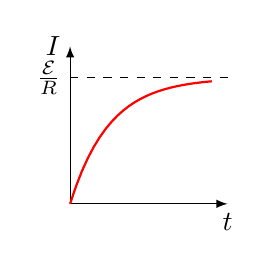
\begin{tikzpicture}[>=latex]
					\draw[->] (0,0) -- ++(2,0) node[below] {$t$};
					\draw[->] (0,0) -- ++(0,2) node[left] {$I$};
					\node[left] at (0, 1.6) {$\frac{\mathcal{E}}{R}$};
					\draw[dashed] (0, 1.6) -- ++(2,0);
					\draw[domain=0:1.8, red, thick] plot (\x, {1.6*(1-exp(-2*\x))});
				\end{tikzpicture}
			\end{column}
			\begin{column}{0.7\linewidth}
				\begin{block}{}
					Закон Ома для кола $\mathcal{E} + \mathcal{E}_\text{si} = IR$. Враховуючи що $\mathcal{E}_\text{si} = -L dI/dt$, закон набуде вигляду
					\begin{equation*}
						L\frac{dI}{dt}  + IR = \mathcal{E}.
					\end{equation*}
					Після інтегрування ми отримаємо:
					\begin{equation*}
						I(t) = \frac{\mathcal{E}}{R}\left(1 - e^{-\frac{R}{L}t} \right) ,
					\end{equation*}
					де $\tau = \frac{L}{R}$ --- називають \alert{часом релаксації}.
				\end{block}
			\end{column}
		\end{columns}
	\end{onlyenv}
	\framesubtitle<2>{Екстраструми при розмиканні}
	\begin{onlyenv}<2>
		\begin{columns}
			\begin{column}{0.25\linewidth}\centering
				\begin{circuitikz}[
						resistor = european,
						scale=0.7, transform shape]
					\draw (0,0) -- (0,1) coordinate (A) -- (0, 2) to[R, l=$R$] (3, 2) -- (3,1) coordinate (A') -- (3, 0);
					\draw (3, 0) to[battery2, l=$\mathcal{E}$] (1.5, 0) to[opening switch, l=$S$, mirror]  (0, 0);
					\draw (A) to[L, l={$L$, $r$}] (A');
					%					\draw
					%					(0,0) to[battery2, l=$\mathcal{E}$] ++(0,2)  to[R, l=$R$] ++(2.5, 0) to[L, l=$L$] ++(0, -2)
					%					to[opening switch, l=$S$, mirror] ++(-2.5, 0) -- cycle
					%					;
				\end{circuitikz}
				\begin{tikzpicture}[>=latex]
					\draw[->] (0,0) -- ++(2,0) node[below] {$t$};
					\draw[->] (0,0) -- ++(0,2) node[left] {$I$};
					\node[left] at (0, 1.6) {$I_0$};
					\draw[domain=0:1.8, red, thick] plot (\x, {1.6*exp(-1.5*\x)});
				\end{tikzpicture}
			\end{column}
			\begin{column}{0.75\linewidth}
				\begin{block}{}\justifying
					Спочатку ключ $S$ замкнутий. Тоді через опір $R$ і через котушку індуктивності $L$ тече струм:
					\begin{equation*}
						I_0 = \mathcal{E} / r.
					\end{equation*}
					Після розмикання ключа (відключення ЕРС) магнітне поле почне убувати. Це збудить електрорушійну $\mathcal{E}_\text{si}$ силу та
					індукційний струм $I$ у контурі. Такий струм називається \alert{екстраструмом розмикання}. По закону Ома:
					\begin{equation*}
						I(R+r) = -L\frac{dI}{dt}.
					\end{equation*}
					Після інтегрування ми отримаємо:
					\(
					I(t) = I_0e^{-\frac{R + r}{L}t}.
					\)
				\end{block}
			\end{column}
		\end{columns}
		\begin{block}{}\justifying\footnotesize
			Якщо $R \gg r$, то $\mathcal{E}_\text{si} = \frac{R}{r}\mathcal{E}e^{-\frac{R}{L}t}$.  При розмиканні ця величина може
			значно перевершити ЕРС батареї, тобто може статись пробій, що спостерігається під час вимкнення струму в колах з великими
			індуктивностями.
		\end{block}
	\end{onlyenv}
\end{frame}
% ===========================================================================

%% --------------------------------------------------------
\section{Взаємна індукція}
%% --------------------------------------------------------



% ============================== Слайд ## ===================================
\begin{frame}{Взаємна індукція}{}
	\begin{columns}
		\begin{column}{0.4\linewidth}\centering
			\input{tikz/12contours.tikz}
		\end{column}
		\begin{column}{0.6\linewidth}
			\begin{overprint}
				\onslide<1>
				\begin{block}{}\justifying
					Нехай два нерухомих контури $1$ і $2$ розташовані близько один до одного. Якщо в контурі $1$ тече струм $I_1$, він створює через контур
					$2$ магнітний потік $\Phi_2$, пропорційний струму $I_1$:
					\begin{equation*}
						\Phi_{21} = \frac1c L_{21}I_1
					\end{equation*}
					Аналогічно, якщо в контурі $2$ тече струм $I_2$, то він створює через контур $1$ магнітний потік:
					\begin{equation*}
						\Phi_{12} = \frac1c L_{12}I_2.
					\end{equation*}
				\end{block}
				\onslide<2>
				\begin{block}{}\justifying
					Закони Ома для контурів:
					\begin{equation*}
						\begin{cases}
							I_1R_1 = \mathcal{E}_1 - \dfrac1{c^2}\dfrac{d}{dt}\left( L_{11} I_1\right) - \dfrac1{c^2}\dfrac{d}{dt}\left( L_{12} I_2\right),
							\\[1,5ex]
							I_2R_2 = \mathcal{E}_2 - \dfrac1{c^2}\dfrac{d}{dt}\left( L_{21} I_1\right) - \dfrac1{c^2}\dfrac{d}{dt}\left( L_{22} I_2\right).
						\end{cases}
					\end{equation*}
					Наявність магнітного зв'язку між контурами проявляється в тому, що за будь-якої зміни струму в одному з контурів в іншому контурі виникає
					ЕРС індукції. е явище називають \alert{взаємною індукцією}.
				\end{block}
			\end{overprint}
		\end{column}
	\end{columns}
	\begin{overprint}
		\onslide<1>
		\begin{block}{}\justifying
			Коефіцієнти пропорційності $L_{12}$ і $L_{21}$ називають \alert{коефіцієнтами взаємної індуктивністю} контурів.
		\end{block}
		\onslide<2>
		\begin{block}{}\justifying
			$L_{12}$ --- алгебраїчна величина, яка може мати різний знак, а також дорівнювати нулю.
		\end{block}
	\end{overprint}
\end{frame}
% ===========================================================================




% ============================== Слайд ## ===================================
\begin{frame}{Розрахунок коефіцієнтів взаємної індуктивності}{}
	\begin{exampleblock}{\small Приклад}\justifying\scriptsize
		Довгий парамагнітний циліндр об'ємом $V$ має дві обмотки (одна на іншій). Одна обмотка містить $n_1$ витків на одиницю довжини, інша ---
		$n_2$. Знайдемо їхню взаємну індуктивність, нехтуючи крайовими ефектами.
	\end{exampleblock}

	\begin{overprint}
		\onslide<1>
		\begin{block}{\small Розв'язок}\justifying\scriptsize
			Оскільки $L_{21} = \Phi_2 / I_1$. Це означає, що ми повинні створити струм $I_1$ в обмотці $1$ і обчислити повний магнітний потік через всі витки
			обмотки $2$. Якщо в обмотці $2$ міститься $N_2$ витків, то
			\[
				\Phi_2 = N_2 B_1 S,
			\]
			де $S$ --- площа поперечного перерізу циліндра. Оскільки $N_2 = n_2 l$, $l$ --- довжина циліндра, $B_1 = \frac{4\pi}{c} \mu n_1 I_1$, то
			\[
				\Phi_2 =  \frac{4\pi}{c} \mu N_2 n_1 I_1 S.
			\]
			Отже
			\[
				L_{21} = \frac{4\pi}{c} \mu \frac{N_2 N_1}{l} S.
			\]
			Аналогічно знаходимо і $L_{12}$:
			\[
				L_{12} = \frac{4\pi}{c} \mu \frac{N_1 N_2}{l} S.
			\]
		\end{block}
		\onslide<2>
		\begin{block}{\small Зауваження}\justifying\scriptsize
			В розглянутому прикладі коефіцієнти індуктивності задовольняють співвідношенням:
			\begin{equation*}
				L_{21} = L_{12} = \sqrt{L_1L_2}
			\end{equation*}
			Їх справедливість пов'язана, по-перше, з тим, що ми знехтували розсіюванням магнітного потоку, а по-друге, з тим, що магнітна проникність осердя не
			залежить від величини магнітного поля. Співвідношення $L_{21} = L_{12}$ не буде виконуватись для феромагнетика, для якого  $\mu = \mu(H)$ і за умови що
			$N_1 \neq N_2$. Тоді обмотки при однакових струмах створюють в осерді різні магнітні поля, так що вирази для $L_{21}$ і $L_{12}$ міститимуть різні
			коефіцієнти $\mu$, що й
			призводить до нерівності.
		\end{block}
	\end{overprint}
\end{frame}
% ===========================================================================




% ============================== Слайд ## ===================================
\begin{frame}{Теорема взаємності}{}
	\begin{block}{}\justifying
		Теоремою взаємності стверджує, що коефіцієнтами взаємної індуктивністю контурів однаков:
		\begin{equation*}
			\tcbhighmath{L_{12} = L_{21}.}
		\end{equation*}
		Завдяки цій теоремі можна не робити різниці між $L_{12}$ і $L_{21}$ і просто говорити про взаємну індуктивність двох контурів.
	\end{block}

	\begin{block}{Практичне застосування}\justifying
		Практичне застосування теореми взаємності полягає у тому, що якщо по контурам течуть однакові струми $I$, то
		\begin{equation*}
			\Phi_1 = \Phi_2
		\end{equation*}
		Ця обставина нерідко дає змогу сильно спрощувати вирішення питання про знаходження, наприклад, магнітних потоків.
	\end{block}
\end{frame}
% ===========================================================================



% ============================== Слайд ## ===================================
\begin{frame}{Задачі на застосування теореми взаємності}{}\scriptsize
	\begin{exampleblock}{\small Задача 1}\justifying
		Два тонкі колові провідники, осі яких співпадають, лежать в одній площині. Радіус зовнішнього провідника $R_1$ внутрішнього $R_2$ ($R_2 \ll
			R_1$). Знайдіть магнітний потік, що пронизує площу зовнішнього провідника, якщо по внутрішньому провіднику тече струм~$I$.
	\end{exampleblock}
	\begin{exampleblock}{\small Задача 2}\justifying
		Магнітний диполь з моментом $p_m$ обертається з частотою $\omega$ навколо осі, яка проходить через його центр і перпендикулярна магнітному моменту
		(див. рис.). Знайти струм в плоскому нерухомому кільці радіусом $a$ з опором $R$, яке знаходиться на відстані $l \gg a$ від
		диполя. Нормаль $\vect{n}$ до площини кільця перпендикулярна осі обертання диполя. Самоіндукцією рамки знехтувати.
	\end{exampleblock}
	%---------------------------------------------------------
	\begin{columns}
		\begin{column}{0.5\linewidth}\centering
			\begin{tikzpicture}[rotate=90]
				\draw[red!40, ultra thick] (0, 0) [partial ellipse=0:360:0.6 and 2];
				\draw[arrowpos={0.5}{2pt}{7pt}, red!40, ultra thick] (0, 0) [partial ellipse=0:360:0.2 and 0.6];
			\end{tikzpicture}
		\end{column}
		\begin{column}{0.5\linewidth}\centering
			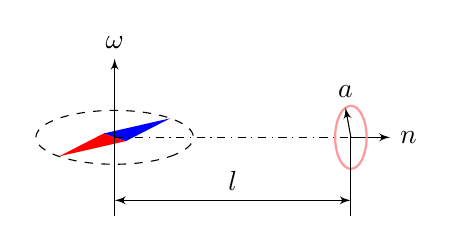
\begin{tikzpicture}[scale=1]
				\tdplotsetmaincoords{0}{0}
				\begin{scope}[tdplot_main_coords, rotate around x=70, rotate around z=-45]
					\draw [dashed] (0,0,0) circle (1);
					\fill [blue] (180:0.2) -- (90:1) -- (0:0.2) -- cycle;
					\fill [red] (180:0.2) -- (-90:1) -- (0:0.2) -- cycle;
				\end{scope}
				\draw [-latex'] (0,-1) -- (0,1) node [above] {$\omega$};
				\draw [-latex'] (3,0) -- (3.5,0) node [right] {$\vect{n}$};
				\begin{scope}[shift={(3,0,0)}, tdplot_main_coords, rotate around y=60]
					\draw [thick, red!40] (0,0,0) circle (0.4);
					\draw [-latex'] (0,0) -- +(110:0.4) node[above] {$a$};
				\end{scope}
				\draw (3,0) -- ([yshift=-1cm]3,0);
				\draw [dash dot] (0,0) -- (3,0);
				\draw [latex'-latex']  (0,-0.8) -- node [above] {$l$}(3,-0.8);
			\end{tikzpicture}
		\end{column}
	\end{columns}
	%---------------------------------------------------------
\end{frame}
% ===========================================================================


%% --------------------------------------------------------
\subsection{Принцип роботи трансформаторів}
%% --------------------------------------------------------


% ============================== Слайд ## ===================================
\begin{frame}{Трансформатор}{}
	\framesubtitle<1>{Принцип роботи}
	\framesubtitle<2>{Теорія}
	\begin{onlyenv}<1>
		\begin{block}{}
			Принцип дії трансформаторів --- пристроїв, що застосовуються для підвищення або зниження напруги змінного струму, заснований на явищі взаємної індукції.
		\end{block}
		\begin{columns}
			\begin{column}{0.4\linewidth}\centering
				\includegraphics[width=0.85\linewidth]{Transformator}
			\end{column}
			\begin{column}{0.6\linewidth}
				\begin{block}{}\justifying
					Первинна і вторинна обмотки з $N_1$ і $N_2$ витками укріплені на замкнутому залізному осерді. Змінна напруга $\mathcal{E}_1$ у первинній
					обмотці створює струм $I_1$ і змінний магнітний потік $\Phi$, локалізований в осерді. Потік пронизує витки вторинної обмотки, викликаючи ЕРС
					взаємної індукції, а в первинній — ЕРС самоіндукції.
				\end{block}
			\end{column}
		\end{columns}
	\end{onlyenv}
	\begin{onlyenv}<2>
		\begin{block}{}\small\justifying
			Струм $I_1$ у первинній обмотці визначається за законом Ома:
			\begin{equation*}
				\mathcal{E}_1 - \frac{d}{dt}(N_1\Phi) = I_1R_1.
			\end{equation*}
			При швидкозмінних полях $I_1R_1 \ll \mathcal{E}_1, \frac{d}{dt}(N_1\Phi)$:
			\begin{equation*}
				\mathcal{E}_1 \approx N_1 \frac{d\Phi}{dt}.
			\end{equation*}

			ЕРС у вторинній обмотці:
			\begin{equation*}
				\mathcal{E}_2 = -N_2 \frac{d\Phi}{dt} = -\frac{N_2}{N_1} \mathcal{E}_1,\quad \text{\scriptsize знак «$-$» вказує на протилежність фаз.}
			\end{equation*}
			Відношення $\eta = \frac{N_2}{N_1}$ називається \alert{коефіцієнтом трансформації}.
		\end{block}
		\begin{block}{}\justifying\scriptsize
			Якщо $\eta > 1$, то це підвищувальний трансформатор, що збільшує ЕРС і зменшує струм.

			\smallskip

			Якщо $\eta < 1$, то це знижувальний трансформатор, що зменшує ЕРС і збільшує струм.
		\end{block}
	\end{onlyenv}
\end{frame}
% ===========================================================================



%% --------------------------------------------------------
\section{Енергія магнітного поля}
%% --------------------------------------------------------



% ============================== Слайд ## ===================================
\begin{frame}{Енергія магнітного поля}{}
	\begin{onlyenv}<1>
		\begin{block}{}\justifying
			Провідник зі струмом створює магнітне поле, яке з'являється та зникає разом зі струмом. \alert{Магнітне поле є носієм енергії}, що дорівнює
			роботі струму на його створення. Розглянемо роботу, яку виконує джерело при замиканні ключа в колі по переміщенню заряду $dq = Idt$:
		\end{block}
		\begin{columns}
			\begin{column}{0.3\linewidth}\centering
				\begin{circuitikz}[
						scale=0.7, transform shape]
					\draw
					(0,0) to[L, l=$L$] ++(0,2) to[battery2, l=$\mathcal{E}$] ++(2.5, 0) to[R, l=$R$] ++(0, -2)
					to[closing switch, l=$S$, mirror] ++(-2.5, 0) -- cycle
					;
				\end{circuitikz}
			\end{column}
			\begin{column}{0.7\linewidth}
				\begin{block}{}\justifying
					\begin{multline*}
						\delta A = \mathcal{E} dq = I^2Rdt - \mathcal{E}_\text{si}Idt = \\
						= \underbrace{I^2Rdt}_\text{Теплота} +
						\underbrace{\frac1{c^2}LIdI}_\text{\parbox{2.2cm}{\centering\scriptsize\strut\ignorespaces Енергія\\ магнітного\\
								поля}}.
					\end{multline*}
				\end{block}
			\end{column}
		\end{columns}
		\begin{block}{}\justifying
			Енергія магнітного поля:
			\(
			W = \frac1{c^2}\int\limits_0^I LIdI = \frac1{c^2}\frac{LI^2}{2} = \frac1c I\Phi = \frac{\Phi^2}{2L}.
			\)
		\end{block}
	\end{onlyenv}
	\begin{onlyenv}<2-3>
		\begin{block}{}
			Енергію магнітного поля визначається через характеристики поля.
		\end{block}
		\vspace*{-2ex}
		\begin{columns}\small
			\begin{column}{0.25\linewidth}\centering
				\includegraphics[width=0.75\linewidth]{tikz/Solenoid.pdf}
			\end{column}
			\begin{column}{0.75\linewidth}
				\begin{block}{}
					Розглянемо однорідне магнітне поле всередині довгого соленоїда.\\[1ex]

					Індуктивність соленоїда:
					\begin{equation*}
						L= \frac{4\pi\mu N^2 S}{l}.
					\end{equation*}
					Магнітне поле в середині соленоїда:
					\begin{equation*}
						B = \dfrac{4\pi\mu NI}{c l}
					\end{equation*}
				\end{block}
			\end{column}
		\end{columns}
	\end{onlyenv}
	\vspace*{-2ex}
	\begin{overprint}
		\onslide<2>
		\begin{block}{}\justifying
			Енергія магнітного поля:
			\begin{equation*}
				W =  \frac1{c^2}\frac{LI^2}{2} = \frac1{c^2}\frac{(4\pi\mu N I)^2 S l }{ 8\pi\mu l^2} = \frac{B^2}{8\pi\mu} V = \frac{BH}{8\pi}
				V.
			\end{equation*}
		\end{block}
		\onslide<3>
		\begin{block}{}\justifying
			Густина енергії магнітного поля:
			\(
			\tcbhighmath{w =  \frac{BH}{8\pi}.}
			\)\\[1ex]

			\alert{Магнітна енергія зосереджена в об'ємі соленоїда --- в тій області простору, де присутнє магнітне поле}.
		\end{block}
	\end{overprint}
\end{frame}
% ===========================================================================



% ============================== Слайд ## ===================================
%\begin{frame}{Енергія магнітного поля (загальний випадок)}\small
%\framesubtitle<1>{Попередні зауваження}
%\begin{onlyenv}<1>
%\begin{block}{}\justifying
%    Наведемо тепер загальне виведення виразу для енергії, який не обмежений будь-яким конкретним класом систем, на зразок соленоїда.
%
%\bigskip
%
%Саме \alert{магнітне поле роботи над зарядами не виконує}, а \alert{виконує її вихрове електричне поле}, що виникає (за законом індукції)
%на
%стадії
%<<включення>> магнітного поля.
%
%\end{block}
%\end{onlyenv}
%\begin{onlyenv}<2>
%\begin{block}{}\justifying
%    За законом Джоуля-Ленца робота електричного поля $\Efield$ над струмами $\vect{j}$ в одиничному об'ємі в одиницю часу дорівнює
%    $\vect{j}\cdot\Efield$. Відповідно за час $dt$ в об'ємі $V$ робота сил поля дорівнює:
%\begin{equation*}
%    \delta A = dt \iiint\limits_V \vect{j}\cdot\Efield dV.
%\end{equation*}
%З теореми про циркуляцію (у диференціальній формі) $\vect{j} = \frac{c}{4\pi} \Rot\Hfield$, а тому робота поля:
%\begin{equation*}
%    \delta A = \frac{cdt}{4\pi} \iiint\limits_V \Efield\cdot\Rot\Hfield dV.
%\end{equation*}
%З урахуванням тотожності $\Div(\Efield\times\Hfield) = \Hfield\cdot\Rot\Efield-\Efield\cdot\Rot\Hfield$ перепишемо вираз для роботи:
%\begin{equation*}
%    \delta A = \frac{cdt}{4\pi} \iiint\limits_V \left[\Hfield\cdot\Rot\Efield-\Div(\Efield\times\Hfield)\right] dV.
%\end{equation*}
%\end{block}
%\end{onlyenv}
%\begin{onlyenv}<3>
%\begin{block}{}\justifying
%\begin{equation*}
%    \delta A = \frac{cdt}{4\pi} \iiint\limits_V \left[\Hfield\cdot\Rot\Efield-\Div(\Efield\times\Hfield)\right] dV.
%\end{equation*}
%    Другий інтеграл обертається в нуль. Дійсно, перетворюючи об'ємний інтеграл за формулою Остроградського-Гауса в поверхневий і
%враховуючи,
%    що на нескінченно віддаленій поверхні поля обертаються в нуль $\Efield, \Hfield \to 0$, отримаємо
%\begin{equation*}
%    \iiint\limits_V \Div(\Efield\times\Hfield) = \oiint\limits_S (\Efield\times\Hfield) dS = 0.
%\end{equation*}
%Врахуємо також закон електромагнітної індукції $\Rot\Efield = - \frac1c \frac{\partial\Bfield}{\partial t}$:
%\begin{equation*}
%    \delta A = \frac{cdt}{4\pi} \iiint\limits_V \Hfield\cdot\Rot\Efield dV = - \frac{cdt}{4\pi} \iiint\limits_V
%    \Hfield\cdot\frac{\partial\Bfield}{\partial t} dV .
%\end{equation*}
%\end{block}
%\end{onlyenv}
%\end{frame}
% ===========================================================================



%% --------------------------------------------------------
\section{Пондеромоторні сили в магнітному полі}
%% --------------------------------------------------------


% ============================== Слайд ## ===================================
\begin{frame}{Пондеромоторні сили в магнітному полі}{}\small
	\framesubtitle<1>{Закон збереження енергії}
	\begin{center}
		\begin{tikzpicture}[]
			\node[anchor=center, opacity=0.75, ] at (0, 0) {\includegraphics[width=6cm]{pull_in_solenoid}};
		\end{tikzpicture}
	\end{center}
	\begin{overprint}
		\onslide<1>
		\begin{block}{}\justifying
			По \alert{закону збереження енергії} \alert{робота, яку виконують джерела струму}, йде на теплоту, на збільшення магнітної енергії і на
			механічну роботу:
			\begin{equation*}
				\delta A_\text{дж} = \delta Q + dW + \delta A_\text{мех}.
			\end{equation*}
			З іншого боку, та ж робота визначається як:
			\begin{equation*}
				\delta A_\text{дж} = \delta Q - \mathcal{E}_\text{in} I dt,
			\end{equation*}
			Звідки
			\begin{equation*}
				- \mathcal{E}_\text{in} I dt = dW + \delta A_\text{мех}
			\end{equation*}
		\end{block}
		\framesubtitle<2>{Випадок $I = \const$}
		\onslide<2>
		\begin{equation*}
			-\mathcal{E}_\text{in} I dt = dW + \delta A_\text{мех}
		\end{equation*}
		Розглянемо умову, коли в колі підтримується постійним струм.
		\begin{equation*}
			- \mathcal{E}_\text{in} I dt = + \frac{I^2}{c^2} dL.
		\end{equation*}
		При цьому, зміна магнітної енергії $dW = \frac{I^2}{2c^2} dL$. Отже, $\delta A_\text{мех} = + dW$, а сила втягування:
		\begin{equation*}
			F_x = + \left( \frac{d W}{dx} \right)_{I}
		\end{equation*}
		\framesubtitle<3>{Випадок $\Phi = \const$}
		\onslide<3>
		\begin{equation*}
			-\mathcal{E}_\text{in} I dt = dW + \delta A_\text{мех}
		\end{equation*}
		Розглянемо умову, коли в колі підтримується потік, що пронизує котушку (наприклад якщо котушка із надпровідника).
		\begin{equation*}
			- \mathcal{E}_\text{in} I dt = 0.
		\end{equation*}
		Отже, $\delta A_\text{мех} = - dW$, а сила втягування:
		\begin{equation*}
			F_x = - \left( \frac{dW}{dx} \right)_{\Phi}
		\end{equation*}
	\end{overprint}
\end{frame}
% ===========================================================================


% ============================== Слайд ## ===================================
\begin{frame}{Приклади}{Поведінка різних тіл в магнітному полі}
	\begin{tblr}{
		colspec = {X[c,m, font=\small]X[c,m, font=\small]}
		}
		\includegraphics[width=0.5\linewidth]{amplula_FeCl}                 & \includegraphics[width=0.5\linewidth]{probirka_FeCl}   \\
		Ампула з парамагнітним розчином хлористого заліза в магнітному полі & Втягування розчину хлористого заліза в магнітне поле   \\
		\includegraphics[width=0.5\linewidth]{palochka_Bi}                  & \includegraphics[width=0.5\linewidth]{Flame_diamagnet} \\
		Діамагнітна паличка вісмута в магнітному полі                       & Діамагнетизм полум'я
	\end{tblr}
\end{frame}
% ===========================================================================



% ============================== Слайд ## ===================================
\begin{frame}{Підйомна сила електромагніта}{}\small
	\begin{columns}
		\begin{column}{0.25\linewidth}
			\includegraphics[width=\linewidth]{electromagnet_force}
		\end{column}
		\begin{column}{0.75\linewidth}
			\begin{block}{}\justifying
				За теоремою про циркуляцію для $\Hfield$:
				\begin{equation*}
					\frac{B}{\mu} l + B\ 2x = \frac{4\pi}{c} IN, \Rightarrow B = \frac{4\pi\mu}{c} \frac{NI}{l + 2\mu x},
				\end{equation*}
				де $l$ --- довжина контура в середині магніту.
				Потік магнітного поля через площу перерізу $S$ магніту:
				\begin{equation*}
					\Phi = NBS = \frac{4\pi\mu}{c} \frac{N^2I}{l + 2\mu x} S.
				\end{equation*}
			\end{block}
		\end{column}
	\end{columns}
	\begin{block}{}\justifying
		За умови, що струм постійний, зміна енергії магнітного поля при віртуальній зміні $x$ дорівнює $dW = \frac{I d\Phi}{2c}$,
		і силу можна знайти як:
		\begin{equation*}
			F_x =  \left( \frac{d W}{dx} \right)_{I} = \frac{I}{2c} \left( \frac{d \Phi}{dx} \right)_{I} = -\frac{4\pi\mu^2}{c^2}\frac{N^2I^2}{(l + 2\mu
				x)^2} S = \frac{B^2}{8\pi} 2S.
		\end{equation*}Сила $F_x <0 $ означає, що це сила притягання.
	\end{block}
\end{frame}
% ===========================================================================

\end{document}
